\textbf{Cited from} \href{https://steemit.com/monero/@luigi1111/understanding-monero-cryptography-privacy-part-2-stealth-addresses}{blog} by \href{https://github.com/luigi1111}{luigi1111}.\par
\begin{displayquote}
This is part two of a series of unknown size; it'll be done when it's done. Part one is \href{https://steemit.com/monero/@luigi1111/understanding-monero-cryptography-privacy-introduction}{here}.\\\\
Part two focuses on stealth addresses, an essential part of the protocol.\\\\
Note: Monero is based on the \href{https://cryptonote.org/whitepaper.pdf}{Cryptonote protocol} -- though it has diverged and will continue to diverge -- along with numerous other coins; much of this series applies equally well to the others with some caveats. Monero is easily the largest and most active Cryptonote-based project.
\end{displayquote}

Hello! I am back with part two of my series on Monero cryptography and privacy; in this series, I'm attempting to make the concepts as easy to understand as possible. I want you to have the same ``lightbulb'' moments I had when I first ``got'' these concepts (my understanding has evolved over a period of time).\par
In part two, we will be discussing stealth addresses, though you may learn some new concepts along the way. Stealth addresses are one of the two complementary techniques used to provide sender/receiver privacy in Monero.\par
So, what are stealth addresses? Well, they look like this:
\begin{figure}[H]
	\centering
	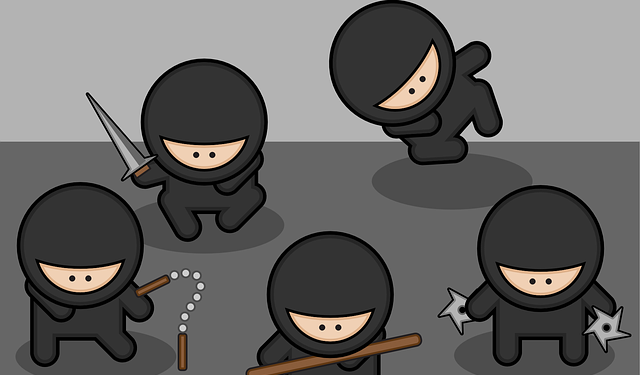
\includegraphics[width=0.8\linewidth]{./images/blog-series/xmr-crypto-luigi1111/stealth-address-kidding.png}
\end{figure}
(just kidding)\par
In my own words, stealth addressing is a technique whereby a \textbf{sender} can take a \textbf{recipient's} public address and transform it to a one-time address such that:
\begin{enumerate}
	\item it is \textbf{publicly unlinkable} to the original public address;
	\item it is \textbf{publicly unlinkable} to \textbf{any} other one-time address;
	\item only the \textbf{recipient} can link all their payments together
	\item only the \textbf{recipient} can derive the secret key associated with the one-time address
\end{enumerate}
Using stealth addressing, a recipient can publish one address and receive unlimited* publicly unlinkable payments.\par

*[The chance of a \href{https://en.wikipedia.org/wiki/Collision_(computer_science)}{collision} (two stealth addresses being the same) is cryptographically negligible. Using the \href{https://en.wikipedia.org/wiki/Birthday_problem}{Birthday Paradox} we can roughly estimate it would take \(\sqrt{l}\), or about \(2^{126}\), stealth addresses being created before having a 50\% chance of a collision. The result would be that the colliding addresses become publicly linkable to each other, but not to any others. There is another, worse problem that would occur in Monero if two stealth addresses were to collide; this will be explained in the ring signature article.\par

For an analogy on how large \(2^{126}\) is, imagine the world has 10 billion people. Each and every person sends a payment to \textbf{every} other person once per \textbf{second}. We would reach \(2^{126}\) payments in about 27 billion \textbf{years}.]\par

Stealth addresses can be implemented by any currency, including Bitcoin, but \textbf{by themselves} do not provide significant extra privacy over avoiding address reuse. However, they are very handy for certain uses, e.g., a published donation address, where address reuse is basically unavoidable.\par

Now you know what stealth addresses \textbf{are}, but you probably don't yet ``get'' them or how they work. Unless you understood previously, in which case why are you reading this article?\par

Before getting into the specifics of stealth addresses in Monero, we need to discuss something:

\subsection{ECDH}
\href{https://en.wikipedia.org/wiki/Elliptic_curve_Diffie%E2%80%93Hellman}{Elliptic Curve Diffie-Hellman} is a variant of the original \href{https://en.wikipedia.org/wiki/Diffie%E2%80%93Hellman_key_exchange}{Diffie-Hellman} key agreement protocol extended for use with \href{https://en.wikipedia.org/wiki/Elliptic_curve_cryptography}{ECC}. In simple terms, two parties can independently generate a shared secret over an unsecured connection (implying that no observer can discover the secret by simply watching their communication). Basic ECDH is quite simple to understand with the application of the scalar multiplication technique from my previous article. For simplicity all key pairs will always be referred to as a lowercase/capital letter (private key \(a\), corresponding public key \(A\), etc).\par

	First, we have Alice. Alice has chosen a random private key (scalar) \(a\) from our group \([1, l-1]\). Her public key is \(A = aG\). \par

	Similarly, Bob chooses random private key \(b\). His public key is \(B = bG\).\par

	Knowing we can add points together, Alice could compute point \(C = A + B\), but so could any observer. \(C\) is \textbf{shared}, but it isn't \textbf{secret}.\par

	Instead, remembering that \(A\) and \(B\) are curve points, and that we can add a point to itself (scalar multiplication!), Alice computes point \(D = aB\). This is just like computing \(B= bG\), but with a different ``base point''. Knowing the result \(D\) and the base \(B\) is no different with respect to helping an observer learn a than knowing result \(A\) and base \(G\)!\par

	Bob, in turn, can also compute \(D' = bA\) (using the apostrophe to be a second ``try'' at the same thing). Now Alice and Bob have a shared, secret point known only to them! \(D = D'\)\par

	In case it isn't clear why Alice's \(D\) equals Bob's \(D'\), here's an example:
	\begin{enumerate}
		\item Use base point \(G\).
		\item Use \(a = 3\); \(A = 3G\).
		\item Use \(b = 4\); \(B = 4G\).
		\item \(a * b = 12\).
		\item ``Alice's'' \(D = aB = 3B = 3*4G = 12G\).
		\item ``Bob's'' \(D' = bA = 4A = 4*3G = 12G\)!
	\end{enumerate}
	Note that \(D\) has a corresponding scalar \(d\) (12 in the above example), that no one knows. We only know it in this case because we know both \(a\) and \(b\)! This isn't particularly useful information, but is the kind of thing I find interesting.

\subsection{Stealth Addresses}
Now that you know about ECDH, let's move on to how \textbf{dual-key stealth addresses} actually work! Again from the \href{https://cryptonote.org/whitepaper.pdf}{Cryptonote whitepaper}, we get:
\begin{figure}[H]
	\centering
	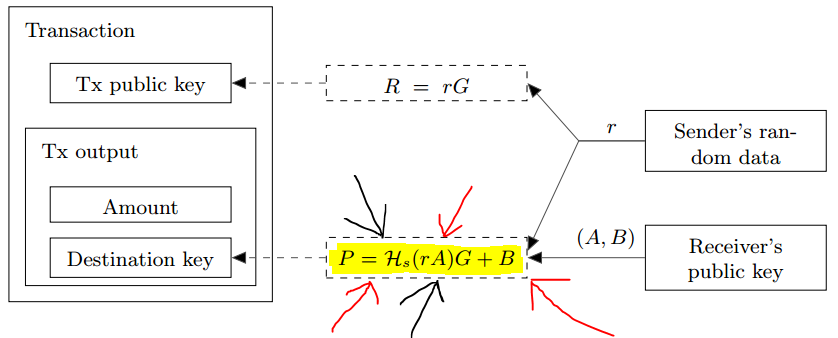
\includegraphics[width=0.8\linewidth]{./images/blog-series/xmr-crypto-luigi1111/stealth-address-cryptenote.png}
\end{figure}

As I've helpfully highlighted and pointed out here, we're looking at \(P = H_s(rA)\cdot G + B\).\par

\textbf{Dual-key} simple refers to the pairs of spend/view keys, which allows ``decoding'' (or removing the unlinkability if you will) stealth addresses \textit{without simultaneously allowing them to be spent}.\par

Now, ignore all that. Let's back up.\par

Alice wants to send a payment to Bob. Alice's \textbf{private spend key} is \(z\), and her \textbf{private view key} is \textbf{y}. Her public address is then \((Z, Y)\) in holy whitepaper order. I've helpfully used letters that aren't referenced above, because \emph{Alice's keys aren't used at all}.\par

Bob's \textbf{public address} is \((A, B)\). Remember from the previous article that the whitepaper helpfully uses \(A\) as the public view key and \(B\) as the public spend key. Presumably Bob's \textbf{private keys} would be \((a, b)\), but Alice (our current perspective) doesn't know them.\par

The final piece needed before ``building'' our first stealth address is \(r\) and \(R\). \(r\) is a new random scalar chosen by Alice for the express purpose of creating a stealth address for Bob. \(R\) is the corresponding curve point for \(rG\). \(r\) is not given to anyone and may be destroyed after use, unless Alice wants to later prove to a 3rd party that she paid Bob. \(R\), however, is added to the transaction for everyone to see. A new \(r\) should be chosen for every single transaction (reusing r to send to the same recipient would result in a stealth address collision!).\par

Here is an example of R at chainradar.com:
\begin{figure}[H]
	\centering
	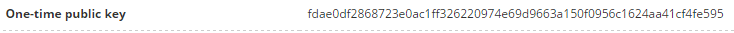
\includegraphics[width=0.8\linewidth]{./images/blog-series/xmr-crypto-luigi1111/R-from-chainradar.png}
\end{figure}

Now that we have our key definitions out of the way, let's create a stealth address! I think walking through the process is the easiest way to understand.\par

\[
	\mathbf{P = H_s(rA)\cdot G+B}
\]

Referenced above we have:
	\begin{enumerate}
		\item \(P\) -- the final \textbf{stealth address} (one-time output key, the destination where funds will actually be sent);
		\item \(H_s\)* -- a \href{https://en.wikipedia.org/wiki/Cryptographic_hash_function}{hashing algorithm} that returns a scalar (i.e., the hash output is interpreted as an integer and reduced modulo \(l\));
		\item \(r\) -- the new random scalar Alice chose for this transaction;
		\item \(A\) -- Bob's \textbf{public view key};
		\item \(G\) -- the standard Ed25519 base point;
		\item \(B\) -- Bob's \textbf{public spend key}.
	\end{enumerate}

	[*Note: the hashing algorithm of choice for Monero and other Cryptonote coins is \href{https://en.wikipedia.org/w/index.php?title=SHA-3&diff=674814400&oldid=674650199#Examples_of_SHA-3_and_Keccak_variants}{keccak-256}. This article's focus is not on hashing algorithms, so if you want to learn more about them please see the linked article. Wikipedia, however, has a good short list of the properties we want:

	\begin{enumerate}
		\item it is quick to compute the hash value for any given message
		\item it is \href{https://en.wikipedia.org/wiki/Computational_complexity_theory#Intractability}{infeasible} to generate a message from its hash value except by trying all possible messages
		\item a small change to a message should change the hash value so extensively that the new hash value appears \textbf{uncorrelated} with the old hash value
		\item it is infeasible to find two different messages with the same hash value
	\end{enumerate}
	\#1 is obvious. \#2 is the one-way property. \#3 is very interesting, as ``uncorrelated'' is quite similar to our magic word, \textbf{unlinkable}. \#4, collision resistance, is very important because a bad algorithm could significantly ``improve'' the chance of a stealth address collision (versus the \(2^{126}\) discussed above).\par

I would add to this list:
	\begin{enumerate}
		\item any length input;
		\item fixed-length output;
		\item output cannot be predicted or chosen in advance (preimage-resistance) -- this is related to \#2 above.]
	\end{enumerate}
Whew, that got long.

\subsubsection{Alright, so let's actually create a stealth address!}
	\begin{enumerate}
		\item Alice does ECDH with her randomly-chosen r and Bob's public view key, \(A\). Let's call this point \textbf{D}. No one other than Alice or Bob can compute \textbf{D} (see the discussion above on ECDH).
		\item Alice uses \(D\) to generate a new scalar; we'll call it \(f\). \(f = H_s(D)\). Yes I like naming things. This is the step that actually \textbf{causes unlinkability} between Bob's outputs (remember \#3 above -- more on this later)!
		\item Alice computes \(F = fG\).
		\item Alice computes \(P = F + B\) (Bob's public spend key).
		\item \(P\) is the stealth destination!
	\end{enumerate}
\subsubsection{Now let's look at Bob's perspective:}
	\begin{enumerate}
		\item Bob receives a transaction; he wants to check if it belongs to him.
		\item Bob retrieves \(R\), which Alice has helpfully attached to the transaction.
		\item Bob computes \(D'\). Note Bob doesn't (yet) know if \(D'\) is equal to \(D\). \(D' = aR\).
		\item Bob computes \(f' = H_s(D')\).
		\item Bob computes \(F' = f'G\).
		\item Bob computes \(P' = F' + B\).
		\item Bob checks if \(P'\) is equal to \(P\), which was included in the transaction as the destination. If yes, Bob realizes he's been paid and does some additional steps (below). If no, Bob ignores the transaction.
	\end{enumerate}
\subsubsection{Some notes:}
	\begin{enumerate}
		\item Computing \(D\) and \(D'\) requires secret data: either \(r\) (Alice) or \(a\) (Bob). Thus, external observers are prevented from proceeding past Alice's step 1. Furthermore, because \(r\) is randomly chosen, even if the observer suspects Alice is sending to Bob's public address (which the observer knows), due to the ECDLP they still can't link this address to \(P\) without knowledge of \(r\) or \(a\) (or pedantically the later steps' values, namely \(D\) and \(f\)).
		\item You may have noticed that this scheme only gives Alice one output for Bob per \(r\), but with auto-denomination Monero and other Cryptonote coins have many outputs per transaction. To get different stealth addresses for each output, Alice (and Bob) append an ``output index'' (an output's position in the transaction: 0, 1, 2, etc.) to \(D\) before hashing it to create the secret shared scalar f. This is a bit of a clarification to Alice's step 2 on \textbf{unlinkability}. That is, while the shared secret \(D\) is already unlinkable to observers, appending an output index allows ``unlimited'' additional unlinkable outputs to be created from one shared secret (see point 3 in the hash section).
		\item Back to the \textbf{dual-key} concept, Bob (or someone working on his behalf with knowledge of \(a\) and \(B\)) can ``scan'' for and detect/link outputs without knowledge of \(b\), which is required below to actually spend that output. The whitepaper calls \((a,B)\) the ``tracking key''.
		\item It is possible to do a non-dual-key stealth addressing scheme, but you must make one of two trade-offs. You can either: 
			\begin{itemize}
				\item use the concept in the whitepaper called a \textbf{truncated address}, which means the view key pair is publicly known and all incoming transactions can be linked (\(a = Hs(B)\)); or 
				\item forego a view key pair entirely, which means scanning requires spending ability (\(P = Hs(rB)\cdot G + B)\)).
			\end{itemize}
	\end{enumerate}
\subsubsection{Bob's Additional Steps}
So, Bob has determined some outputs in a transaction belong to him. Now what does he do? I can imagine two things he \emph{wants} to do: check if this output has already been spent, and (later) actually spend the output. To do either of these things, Bob must first compute the secret key associated with that output (the one-time secret key, \(x\)).
	\begin{enumerate}
		\item Bob recomputes \(f' = Hs(D')\) (as above).
		\item Bob derives \(x = f' + b\) (\(b\) is Bob's private spend key). The ``neat'' thing is that \(P = xG\)! Adding scalars (or points) together preserves linearity. \(P = xG = (f' + b)\cdot G = F' + B\)
		\item To check if \(P\) is spent, Bob computes its ``key image'' and queries the blockchain to see if it is marked as spent. Key image \(I = xH_p(P)\). This will be better explained in the ring signature article. \emph{Fear not!}
		\item To spend \(P\), Bob needs to sign a new transaction with \(x\) (also detailed in the ring signature article).
	\end{enumerate}

	\textbf{[Skip the next section if you hate fun.]}
\subsection{FUN}
\textbf{Now, let's do a ``fun'' exercise with real values for illustration.} \emph{Great...}\par

I'll be using functions that are available in Javascript \href{https://xmr.llcoins.net/}{here}. Doing so allows the curious and discerning reader (\textit{that's you, presumably}) to easily reproduce the results with only a web browser. If you go to the link above and open your browser's console (right-click the page->Inspect, then Console tab), you can enter or copy/paste all the commands below to ``see it in action''. All letters and step numbers match those  above. The scalars b and r below were randomly generated with \code{random_scalar()}; (you obviously can't randomly generate your own if you want to reproduce my results!). You can see the contents of a variable by just typing its name and pressing . ``//'' is a comment in Javascript.\par

Here is the Chrome console:
\begin{figure}[H]
	\centering
	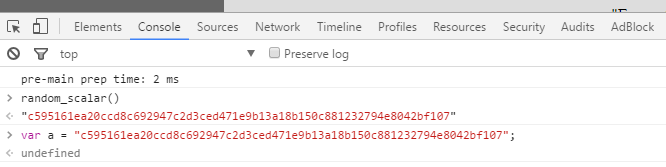
\includegraphics[width=0.8\linewidth]{./images/blog-series/xmr-crypto-luigi1111/stealth-address-chrome-console.png}
\end{figure}

\subsubsection{Preliminary}
\begin{lstlisting}
//Bob's private spend key
 var b = "c595161ea20ccd8c692947c2d3ced471e9b13a18b150c881232794e8042bf107"; 

//Bob's private view key (deterministic derivation); 
//a = "fadf3558b700b88936113be1e5342245bd68a6b1deeb496000c4148ad4b61f02"
var a = hash_to_scalar(b); 

//Bob's public spend key, this function multiplies base G by its input; 
//B = "3bcb82eecc13739b463b386fc1ed991386a046b478bf4864673ca0a229c3cec1"
var B = sec_key_to_pub(b); 

//Bob's public view key; 
//A = "6bb8297dc3b54407ac78ffa4efa4afbe5f1806e5e41aa56ae98c2fe53032bb4b"
var A = sec_key_to_pub(a); 

//returns Bob's public address (for curiosity only), 
//"43tXwm6UNNvSyMdHU4Jfeg4GRgU7KEVAfHo3B5RrXYMjZMRaowr68y12HSo14wv2qcYqqpG1U5AHrJtBdFHKPDE A9UxK6Hy"
pubkeys_to_string(B,A); 

var r = "c91ae3053f640fcad393fb6c74ad9f064c25314c8993c5545306154e070b1f0f";

//R = "396fc23bc389046b214087a9522c0fbd673d2f3f00ab9768f35fa52f953fef22"
var R = sec_key_to_pub(r); 
\end{lstlisting}
\subsubsection{Alice}
\begin{lstlisting}
//ECDH, rA; D = "a1d198629fadc698b48f33dc2e280301679ab2c75a76974fd185ba66ab8418cc"
var D = generate_key_derivation(\(A\), r); 

//0 is the output index; the standard method combines these last few steps into one, but I split them for clarity; 
// f = "bf1d230a09bfdb0bc7fe04cddf8c1635d0ebaaf159ef85dc408ae60879752509"
var f = derivation_to_scalar(D, 0); 

//F = "3e4b39c5b5110d6fbdb77fbcd203709c19fefd28c982a86bda3f3d35fc099738"
var F = sec_key_to_pub(f); 

//``ge'' means group element; this function adds two points together. 
//P = "6cabaac48d3b9043525a703e9e5feb72132f69ea6deca9b4acf9228beb74cd8f"
var P = ge_add(F,B); 
\end{lstlisting}
\subsubsection{Bob}
\begin{lstlisting}
N/A
N/A
var D1 = generate_key_derivation(R, a); //D1 = same as above!
var f1 = derivation_to_scalar(D1, 0); //f1 = same as above!
var F1 = sec_key_to_pub(f1); //F1 = same as above!
var P1 = ge_add(F1,B); //P1 = same as above!
\end{lstlisting}
\subsubsection{Bob's additional steps}
\begin{lstlisting}
N/A

//"sc" means scalar; this function adds two scalars together. 
// x = "97df43cb906896405a8b54ecd4610c92b99de5090b404e5e64b17af17da01601". Now for fun enter sec_key_to_pub(x); and compare with P.
var x = sc_add(f1,b); 

//This combines "hash_to_ec" (Hp, hash to a curve point) and a scalar multiplication of that new point by x. 
// I = "2ba7ee37314d4a1edbeef727f49099c79d55797570cb1206ee2685c94b6550b1" 
// For fun -- spent status
var I = generate_key_image_2(P, x);9 
N/A
\end{lstlisting}
Whew!

\textbf{[End skip.]}
\begin{figure}[H]
	\centering
	
\includegraphics[width=0.8\linewidth]{./images/blog-series/xmr-crypto-luigi1111/tired-dog.jpg}
\end{figure}
tl;dr (\emph{You get one this time!}), stealth addressing allows senders to create ``unlimited'' one-time destination addresses on behalf of the recipient (without any interaction). They can only be recovered and spent by the recipient and can't be publicly linked to each other or the standard address from which they were derived.\par

Until next time!
